%%%%%%%%%%%%%%%%%%%%%%%%%%%%%%%%%%%%%%%%%%%%%%%%%%%%%%%%%%%%%%%%
\begin{figure}[ht]
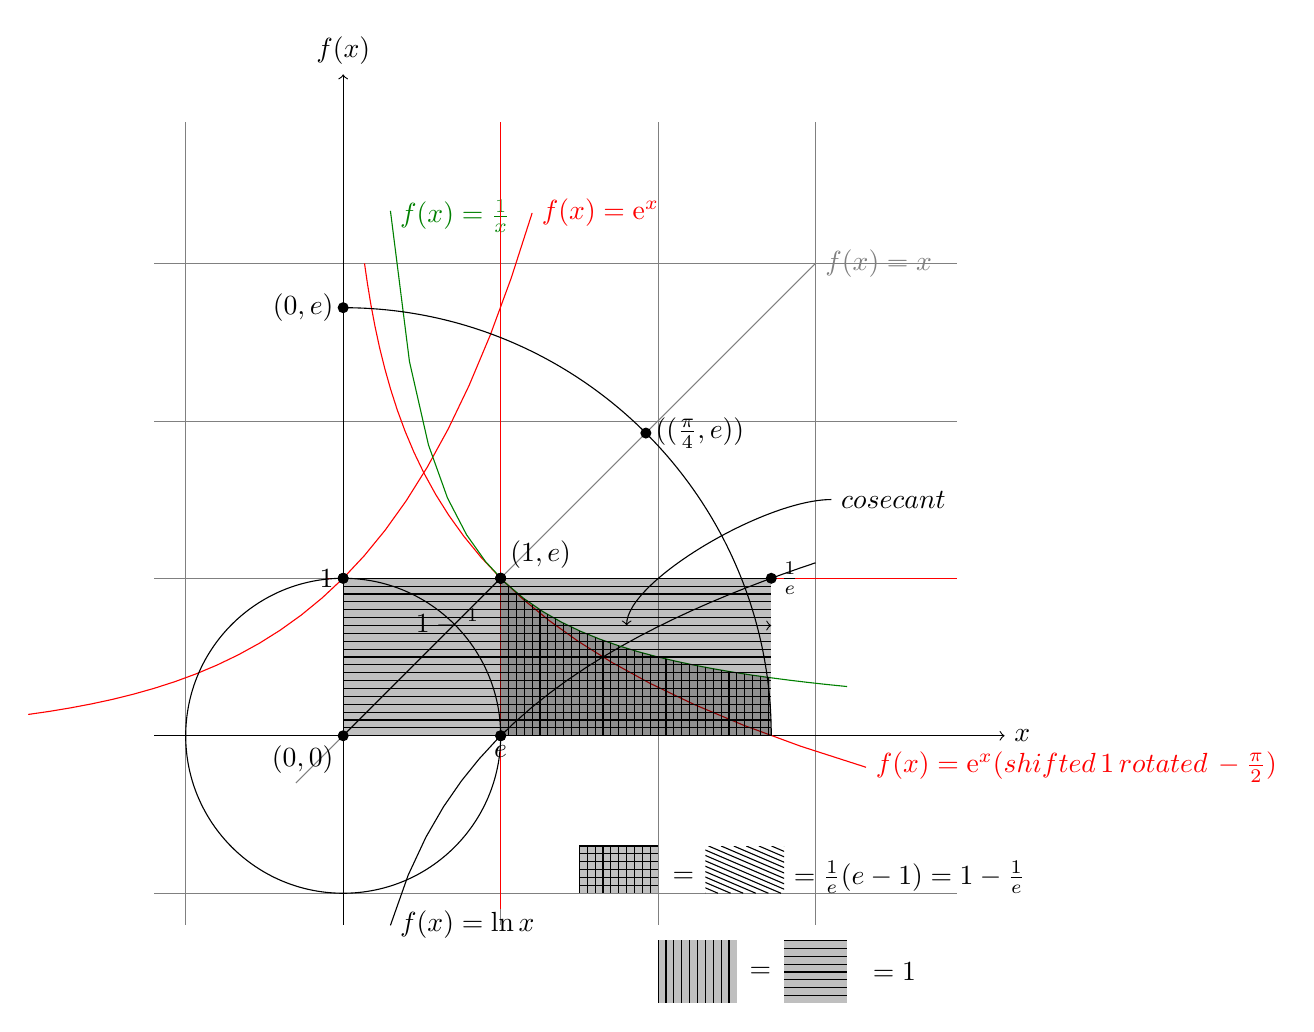
\begin{tikzpicture}[scale=2,domain=-.3:3]

 \draw[very thin,color=gray] (-1.2,-1.2) grid (3.9,3.9);
  \draw[->] (-1.2,0) -- (4.2,0) node[right] {$x$};
  \draw[->] (0,-1.2) -- (0,4.2) node[above] {$f(x)$};

  %% f(x) = x
  \draw[color=gray] plot (\x,\x) node[right] {$f(x) =x$};

  %% f(x) = ln x
  \draw[domain=.3:3,color=black] plot (\x,{ln(\x)});
  \draw[black] (.3,-1.2) node[right] {$f(x) = \ln x$};

  %% cosecant indicator
  \draw[->,black] (3.1,1.5) node[right] {$cosecant$} .. controls ++(left:12pt) and ++(up:8pt) .. (1.8,0.7);


  %% f(x) = e^x
  \draw[domain=-2:1.2,color=red]
  plot (\x,{exp(\x)}) node[right] {$f(x) = \mathrm e^x$};
  %% shifted and rotated
  \draw[domain=-2:1.2,color=red,xshift=1cm,rotate around={-90:(0,1)}]
  plot (\x,{exp(\x)}) node[right] {$f(x) = \mathrm e^x (shifted\, 1\, rotated\, -\frac{\pi}{2})$};

  %% f(x) = 1/x
  \draw[domain=.3:3.2,color=green!50!black] plot (\x,{(1/\x)});
  \draw[color=green!50!black] (.3,3.3) node[right] {$f(x) = \frac{1}{x}$};
  % \draw[] (1,.3) node[anchor=west] {$\scriptsize 1=\ln e$};

  %% (e,y) axis
  \draw[red] (\e,-1.1) -- (\e, 3.9);

  %% (x,1) axis and label
  \draw[red] (-0.1,1) -- (3.9,1);
  \fill[black] (0,1) node[left] {$1$};


  %% secant
  \draw[] (0,0) -- (\e, 1);

  %% circle
  \draw (0,0) circle (1);

  %% dot origin
  \fill[black] (0,0) node[below left] {$(0,0)$} circle (1pt);

  %% dot (0,e)
 \fill[black] (0,\inve) circle (1pt);

  %% dot (0,1)
  \fill[black] (0,1) circle (1pt);

  %% dot (1,1)
  \fill[black] (1,1) circle (1pt);

  %% dot (1, 1/e)
  \fill[black] (1, \inve) circle (1pt);

  %% label (1,e)
  \fill[black] (1,\e) node[anchor=south west] {$(1,e)$} circle (1pt);

  %% dot (e,0)
  \fill[black] (\e,0) node[below] {$e$} circle (1pt);

  %% dot (e,1)
  \fill[black] (\e,1) circle (1pt);

  %% dot (e, 1,e)
  \fill[black] ({exp(1)}, \inve) circle (1pt) node[anchor=west]
  {$\frac{1}{e}$};

  %% 1 - 1/e label
  \draw[<-] ({exp(1)}, .7) -- (\e+.4,.7) node[anchor=west] {$1-\frac{1}{\e}$};
  % \fill[black] (1,{exp(1)}) node[anchor=south west] {$(1,e)$} circle (1pt);

  %% dot (1,0)
  \fill[black] (1,0) circle (1pt);

  %% 1/x area
  \begin{scope}[domain=1:2.71]
    \clip (1,0)--(1,1) -- plot (\x,{(1/\x)}) -- ({exp(1)},0) -- cycle;
    \fill[opacity=.25] (1,0) -- ({exp(1)},0) -- ({exp(1)},1) -- (1,1);
    \foreach \step in {0,.05,...,4} {
      \pgfmathsetmacro\inc{\step}
      \draw (1+\inc,0) -- (1+\inc,1);
    }
  \end{scope}

  %% area lines
  \fill[opacity=.25] (2,-1.3) rectangle (2.5,-1.7);
  \foreach \step in {0,.05,...,.5} {
    \draw (2+\step,-1.3cm) -- (2+\step,-1.7);
  }

  \draw (2.65,-1.5) node {$=$};

  \fill[opacity=.25] (2.8,-1.3) rectangle (3.2,-1.7);
  \foreach \step in {0,.05,...,.4} {
    \draw (2.8,-1.3-\step) -- (3.2,-1.3-\step);
  }
  %% end 1/x area

  \def\eul{{exp(1)}};
  \def\inveul{\inve};
  %% upper square area lines
  \begin{scope}
    \clip (0,0) rectangle (1,1);
    %% \fill[opacity=.25] (0,0) -- ({exp(1)},0) -- ({exp(1)}, \inve) -- (0,\inve) -- cycle;
    \foreach \step in {0,.07,...,2.5} {
      \pgfmathsetmacro\inc{\step}
      \draw (\step,\inveul) -- (\step-.7,1);
      % \draw (-.5+\inc,0) -- (\inc+3,{exp(1)});
    }
  \end{scope}

  %% area key
  \fill[opacity=.25] (1.5,-.7) rectangle (2,-1);
  \foreach \step in {0,.05,...,.5} {
    %% v lines
    \draw (1.5+\step,-.7) -- (1.5+\step,-1);
  }

  \draw (2.03,-.9) node[anchor=west] {$=$};

  \foreach \step in {0,.05,...,.3} {
    %% h lines
    \draw (1.5,-.7-\step) -- (2,-.7-\step);
  }

  %% slant lines key
  %% \fill[opacity=.25] (2.3,-.7) rectangle (2.8,-1);
  \begin{scope}
    \clip (2.3,-.7) rectangle (2.8,-1);
    %% \fill[opacity=.25] (0,0) -- ({exp(1)},0) -- ({exp(1)}, \inve) -- (0,\inve) -- cycle;
    \foreach \step in {1.6,1.68,...,2.8} {
      \pgfmathsetmacro\inc{\step}
      \draw (\step,-.7) -- (\step+.7,-1);
      % \draw (-.5+\inc,0) -- (\inc+3,{exp(1)});
    }
  \end{scope}

  \draw (2.8,-.9) node[anchor=west] {$= \frac{1}{e}(e-1) = 1-\frac{1}{e}$};

  %%
  \draw (3.5,-1.5) node {$= 1$};

  %% e rectangle
  %% PATTERNS seem to be broken
  %% \draw[pattern=dots] (0,0) -- ({exp(1)},0) -- ({exp(1)}, \inve) -- (0,\inve) -- cycle;
  \begin{scope}
    \clip (0,0) -- ({exp(1)},0) -- ({exp(1)}, \inve) -- (0,\inve) -- cycle;
    \fill[opacity=.25] (0,0) -- ({exp(1)},0) -- ({exp(1)}, \inve) -- (0,\inve) -- cycle;
    \foreach \step in {0,.05,...,4} {
      \pgfmathsetmacro\inc{\step}
      \draw (0,\inc) -- ({exp(1)},\inc);
      % \draw (-.5+\inc,0) -- (\inc+3,{exp(1)});
    }
  \end{scope}

  %% e radius (= focus of hyperbola?)

%  \newlength{\gnat}
%  \setlength{\gnat}{{\eul}*1cm}
  \pgfmathsetmacro\e{exp(1) * 1cm}
%  \pgfmathparse{exp(1)cm} \pgfmathresult \let\e\pgfmathresult
  \draw (\eul,0) arc (0:90:\eul);
  \fill (canvas polar cs:angle=45,radius=\e) circle (1pt) node[anchor=west] {($(\frac{\pi}{4},e)$)};
  \fill (0,\eul) circle (1pt) node[anchor=east] {($0,e$)};

  %% arc e
  draw (1,0) arc (e:1);

\end{tikzpicture}
\end{figure}

%%% Local Variables: 
%%% mode: latex
%%% TeX-master: t
%%% End: 
